% THIS IS SIGPROC-SP.TEX - VERSION 3.1
% WORKS WITH V3.2SP OF ACM_PROC_ARTICLE-SP.CLS
% APRIL 2009
%
% It is an example file showing how to use the 'acm_proc_article-sp.cls' V3.2SP
% LaTeX2e document class file for Conference Proceedings submissions.
% ----------------------------------------------------------------------------------------------------------------
% This .tex file (and associated .cls V3.2SP) *DOES NOT* produce:
%       1) The Permission Statement
%       2) The Conference (location) Info information
%       3) The Copyright Line with ACM data
%       4) Page numbering
% ---------------------------------------------------------------------------------------------------------------
% It is an example which *does* use the .bib file (from which the .bbl file
% is produced).
% REMEMBER HOWEVER: After having produced the .bbl file,
% and prior to final submission,
% you need to 'insert'  your .bbl file into your source .tex file so as to provide
% ONE 'self-contained' source file.
%
% Questions regarding SIGS should be sent to
% Adrienne Griscti ---> griscti@acm.org
%
% Questions/suggestions regarding the guidelines, .tex and .cls files, etc. to
% Gerald Murray ---> murray@hq.acm.org
%
% For tracking purposes - this is V3.1SP - APRIL 2009

\documentclass{acm_proc_article-sp}

\begin{document}

\title{Streamlining text messages in a disaster management system: A Text Mining Approach}
%
% You need the command \numberofauthors to handle the 'placement
% and alignment' of the authors beneath the title.
%
% For aesthetic reasons, we recommend 'three authors at a time'
% i.e. three 'name/affiliation blocks' be placed beneath the title.
%
% NOTE: You are NOT restricted in how many 'rows' of
% "name/affiliations" may appear. We just ask that you restrict
% the number of 'columns' to three.
%
% Because of the available 'opening page real-estate'
% we ask you to refrain from putting more than six authors
% (two rows with three columns) beneath the article title.
% More than six makes the first-page appear very cluttered indeed.
%
% Use the \alignauthor commands to handle the names
% and affiliations for an 'aesthetic maximum' of six authors.
% Add names, affiliations, addresses for
% the seventh etc. author(s) as the argument for the
% \additionalauthors command.
% These 'additional authors' will be output/set for you
% without further effort on your part as the last section in
% the body of your article BEFORE References or any Appendices.

\numberofauthors{8} %  in this sample file, there are a *total*
% of EIGHT authors. SIX appear on the 'first-page' (for formatting
% reasons) and the remaining two appear in the \additionalauthors section.
%
\author{
% You can go ahead and credit any number of authors here,
% e.g. one 'row of three' or two rows (consisting of one row of three
% and a second row of one, two or three).
%
% The command \alignauthor (no curly braces needed) should
% precede each author name, affiliation/snail-mail address and
% e-mail address. Additionally, tag each line of
% affiliation/address with \affaddr, and tag the
% e-mail address with \email.
%
% 1st. author
\alignauthor
Maria Regina Estuar\titlenote{Project Leader of eBayanihan system}\\
       \affaddr{Ateneo de Manila University}\\
       \affaddr{Loyola Heights}\\
       \affaddr{Quezon City, Philippines}\\
       \email{restuar@ateneo.edu}
% 2nd. author
\alignauthor
Hadrian Ang\titlenote{description}\\
       \affaddr{Ateneo de Manila University}\\
       \affaddr{Loyola Heights}\\
       \affaddr{Quezon City, Philippines}\\
       \email{hadrianang@outlook.com}
% 3rd. author
\alignauthor Miguel Palma\titlenote{description.}\\
       \affaddr{Ateneo de Manila University}\\
       \affaddr{Loyola Heights}\\
       \affaddr{Quezon City, Philippines}\\
       \email{miguel.palma@obf.ateneo.edu}
	}	


% There's nothing stopping you putting the seventh, eighth, etc.
% author on the opening page (as the 'third row') but we ask,
% for aesthetic reasons that you place these 'additional authors'
% in the \additional authors block, viz.
\additionalauthors{Additional authors: John Smith (The Th{\o}rv{\"a}ld Group,
email: {\texttt{jsmith@affiliation.org}}) and Julius P.~Kumquat
(The Kumquat Consortium, email: {\texttt{jpkumquat@consortium.net}}).}
\date{30 July 1999}
% Just remember to make sure that the TOTAL number of authors
% is the number that will appear on the first page PLUS the
% number that will appear in the \additionalauthors section.

\maketitle
\begin{abstract}
In developing countries, effectiveness of disaster management systems can be measured through adoption. To ensure that the general public embraces the technology, the design of the system should be technology inclusive. eBayanihan is a nationwide web - mobile participatory disaster management system which captures the human dimension of disaster by allowing ordinary citizens to post incidents as they experience it. This paper discusses possible solutions to problems encountered in the SMS based platform in eBayanihan. Specifically, we address the problem of correcting incorrect syntax. (we will place our solution here).


\end{abstract}

% A category with the (minimum) three required fields
% @Hadrian/Migee: check out the category numbers for text mining, sms based systems, disaster management systems

\category{H.4}{Information Systems Applications}{Miscellaneous}
%A category including the fourth, optional field follows...
\category{D.2.8}{Software Engineering}{Metrics}[complexity measures, performance measures]

\terms{Theory}

\keywords{SMS, text mining, disaster systems} % NOT required for Proceedings

\section{Disasters in the Philippines}
More recently, an average of 19 typhoons enter the area of responsibility with around 6 to 9 making a landfall on Philippine soil \cite{shoemaker1991:typhoons}. In 2014, there was a total of X tropical rainstorms that hit the Philippines causing Y pesos of damage as well as Z loss of lives. In year, the Philippine government through Republic Act No. established the National Disaster Risk Reduction Management Council whose primary role is to enter role here. There are N clusters in this council ranging from enter clusters here. The cluster in Information Communications Technology (ICT) requires managing communication infrastructure as will as delivering information from top down (official news to the public) as well as bottom up (public information to the national level). 

\section{Review of Existing Disaster Information Systems}

In the Philippines, there have been efforts in contributing to the development of disaster management systems and applications to collect and report disaster related information. Discuss systems here.

As of enter 2013, the Philippines received a worldwide rank of 12 in the mobile phone ownership with a ratio of enter ratios here. Since only 30 percent of the mobile users own a smart phone, there is still a need to provide an SMS based application for disaster reporting.

\subsection{Types}

\subsection{Measuring Effectiveness}

\section{SMS based platforms}
\subsection{Design}
The SMS based application was designed to accept reports based on the following syntax:
enter syntax here.

enter technical description of algorithm for receiving, processing and plotting

enter figure of SMS feature phone and SMS app.

enter figure of SMS to eBayanihan

\subsection{Problems}

To send an SMS report to eBayanihan, a specific format has to be followed so that it can be parsed properly by the system. The SMS is then parsed for a keyword, urgency level, barangay, city or municipality and then the actual report. Location information is then extracted from the SMS and used to map the report. 

With this in mind, there are three problems that may occur with an SMS report.
First, the SMS sent may not follow the proper format (there are extra or missing commas). Place example.

Second, keywords and urgency level may be misspelled, thus confusing the system. Place example.

Third, the location extracted may not be geo-locatable, which may occur because a) the names of places are misspelled, b) the place has not yet been mapped by the services used
(Google Maps, Nominatim).

\section{Proposed Solution}
There are two possible approaches in solving the problem, namely by correction and approximation. I will explain further here.

\subsection{Correction}
One possible approach to the problem of erroneous SMS reports is to attempt to correct them. A program first queries the database for new SMS that have been deemed to be wrong. Instead of separating solutions to the first and second problems mentioned above, the group instead decided to solve both simultaneously with the algorithm proposed in ~\ref{trie}. Once the SMS report has been corrected for both spelling and formatting errors, it is once again passed through a regex check. If it passes, information is again extracted and sent via HTTP Post to the geolocation module of eBayanihan. 

The group will first tackle the solution to the misspelled words problem and then explain how its approximate string matching solution can be adapted to solving the formatting problem at the same time. One approach to the misspelled words problem is to find the closest string in the given dictionary and then replacing the string with that one. Afterward, this may then be passed on to the gazetteer query stage. Numerous string similarity and distance metrics allow this kind of approximate matching. Hamming distance, Levenshtein distance, Damerau-Levenshtein distance, Longest Common Subsequence and Longest Common Substring are just some examples of these distance metrics. 

Levenshtein distance, or edit distance, is a commonly used metric in approximate string matching and spelling correction. In Peter Norvig's trials, he claims that around 76\% of errors were within an edit distance of one and 98.9\% were within a distance of two \cite{norvig:howto}. It is defined as the minimum number of operations required to change one string into another. The operations defined are insertion (addition of an extra letter), deletion (removal of a character from the string), and substitution (replacing one character with another). Damerau-Levenshtein distance is an extension of this that keeps the three operations, but adds a fourth one, namely transposition or the flipping of adjacent characters. Damerau   

Since there are only 15 keywords and 2 urgency levels, correcting errors given the dictionary is a simple task of selecting
the word with the smallest edit distance when compared to a certain query. Since only a few comparisons are needed, a straightforward
dynamic programming approach would actually work here. 

\begin{displaymath}
	d_{ij} = \left\{
		\begin{array}{lr}
			d_{i-1,j-1} & for \ a_j = b_i\\
			min \left\{
				\begin{array}{lr}
						d_{i-1,j} + cost_{del} (b_i)\\
						d_{i,j-1} + cost_{ins} (a_j)\\
						d_{i-1,j-1} + cost_{sub} (a_j, b_i)\\
				\end{array}	\right. & for \ a_j \not = b_i\\
		\end{array}
		\right.
\end{displaymath}

To simplify computations, the cost of all operations will be equally set to one. 

While the same approach may be used for the names of places, the dictionary here is a lot larger. With over a thousand cities, over a thousand municipalities and thousands of barangays, a straightforward comparison approach will be too slow (given the O(mn) run time of the dynamic programming approach). To solve this problem of efficiency, the group implemented a solution that involves a trie and dynamic programming.

Another problem arises though: what should the query string in approximate string matching be if the SMS is poorly formatted such that even data boundaries (delimiters, in this case commas, between fields such as keyword and urgency) are blurred? For this specific application, commas in the SMS format may be treated as delimiters to data fields, similar to white spaces in English words. This means correcting the format of the SMS may be reduced to finding boundaries between words. There is no absolute solution to the word boundary problem, but an approximate solution may be sufficient <CITE CHINESE GRAPH PEOPLE>.  To solve this, the entire SMS is used as a query string and then a greedy approach that optimizes based on a scoring function decides when to extract tokens from the query. This is done iteratively until enough tokens have been extracted, as explained in the next subsection. 

\subsubsection{Trie with Dynamic Programming}
\label{trie}
A trie is a tree data structure where nodes can contain different keys pertaining to parts of a word. In this algorithm's case, each node contains a character. By using a trie, redundant computations are prevented, as prefixes to the wide range of words in the dictionary will only have to be involved in the computations once. In other words, the memoization array used in the dynamic programming algorithm is recycled, and carried over to other words with the same prefix.

<ADD PICTURE OF SAMPLE TRIE HERE> 

Instead of simply using Levenshtein distance, the group instead opted to use the string optimal alignment distance function (sometimes known as restricted Damerau-Levenshtein distance). It also counts four operations instead of the three by the Levenshtein distance function, however, a single substring cannot be edited more than once. For example, the Damerau-Levenshtein distance of ``there'' and ``etr'' is two, as one can flip the first and second letters or ``etre'' and then insert an ``h'' in between. Its optimal string alignment distance , however, is three because after the initial transposition of the first two letters, one cannot insert another letter (the substring has already been edited). While more restrictive than Damerau-Levenshtein distance, this metric is sufficient for the purposes of the algorithm (approximate matching of wrongly spelled words). This is what will be referred to from now on when edit distance is mentioned. 

The first step to the algorithm is the construction of the trie. Since the the list of cities, municipalities and barangays is not expected to change very often, a separate program builds the trie, then outputs it to a text file to be read whenever the main algorithm has to be run. This will save time once the program is uploaded to the server, as  the building of the trie is moved to the pre-processing stage.

When the main processing program is run, it first reads the trie and reconstructs it from a given text file. Once the full trie has been constructed, processing may begin. Let $s_1 = \{c_1,c_2,c_3 . . . c_n\}$ be the entire SMS composed of $n$ characters where $c_i$ is the $i_{th}$ character of the string. The string $s_1$ is then used as a parameter to a $computeDP(x)$ function where the parameter $x$ is a designated query string. This function traverses through the entire trie in a DFS fashion, doing computations along the way. 
 
Each node $k$ contains two memoization arrays $k.Lev[n]$ and $k.Lcs[n]$ where $n$ is the length of each array, equal to the length of the query string. These arrays hold the DP table for the corresponding operations according to the recurrence relations below. During this traversal, each node is processed. This processing involves setting its parent node, setting its depth, and then the computation of $Lev[0,1. . . n]$ and $Lcs[0,1. . . n]$ based on its parents. Each node normally contains a single character of some word in the given dictionary used to construct the trie. Let $name(k)$ refer to the character contained in node $k$ while $depth(k)$ is its depth in the trie and $parent(k)$ is its parent according to the DFS traversal. If $name(k) = \$$ then backtracking from $parent(k), parent(parent(k)) . . . root$, appending the names of nodes along the way, will result in a word that is in the dictionary (though in reverse). We let $word(k)$ be the resulting word if we were to backtrack from $k$ to the root of the trie. 

<INSERT RECURRENCE RELATIONS HERE> 

Since any node $y$ such that $name(y) = \$$ denotes a word, then the $Lev$ and $Lcs$ arrays of $parent(y)$ will contain the edit distance and longest common subsequence of the query string $s_1$ along every point $\{c_1,c_2,c_3, . . . c_n\}$ when compared to $word(y)$. During the computation $max(k.Lcs[0,1,...,n])$ and $min(k.Lev[0,1,...,n])$ are stored and then input into a function $f(x,z)$ to produce a score value. This score is then compared with a global maximum score $\forall a : word(a) \in Dictionary$. If a word with the same score, same edit distance and same Lcs as the global maximum is found, the longer string is chosen. For the purposes of this study, a simple scoring function $f(x,z) = \frac{x}{z}$ was used, the ratio between the Lcs and edit distance. If the edit distance is zero, the score is automatically made to be infinity. If $depth(y) > length(s_1) + T$ where $T$ is some constant threshold edit distance provided, the trie traversal may stop. This is because $depth(y)$ denotes the length of $word(y)$ and if that goes above he length of the query string plus the threshold, the proceeding nodes cannot be approximate matches for the query. The point $p$ in the query string at which the maximum score $max( f(Lcs[0,1,...n],Lev[0,1,...n])$ was found is stored for the next step in the algorithm. 

Once the trie has been traversed (at least up to the threshold) and a global maximum score has been computed, the initial query string, $s_1$ in this case, is then cut at point $p$. The $word(y)$ that resulted in the maximum score is then appended to the answer string. The string $s_2 = \{c_{p+1}, c_{p+2}, ... c_n\}$ is then the new query string and is afterward passed into $computeDP(x)$ once again. This is done iteratively until the entire string has been processed (a cut is chosen at the end of the query string). 

The answer string is then returned for post-processing so it can be sent back to the geolocation program. 

\subsection{Edge Cases} 
Because the algorithm takes a greedy approach, maximizing based on only a simple scoring function, there are certain cases when it fails to correct the SMS string and actually comes up with a more incorrect answer. 

\subsection{Approximations}
Text mining is proposed approximation approach in solving the problem. In this approach, the syntax is almost disregarded as input string is tokenized and compared to a lookup table for matching. The difference in this approach is that there is a validation process that happens in every correct or incorrect match so there is a percentage increase or decrease in the matching or relevance score. 

We will use a machine learning classification algo here to tag correct and incorrect match.

\section{Experimentation}
\subsection{Problem1: Incorrect syntax}
\subsection{Problem2: Incorrect keyword or location}
\subsection{Problem3: Location not found}

\section{Results}
\section{Discussion}

\subsubsection{Inline (In-text) Equations}
A formula that appears in the running text is called an
inline or in-text formula.  It is produced by the
\textbf{math} environment, which can be
invoked with the usual \texttt{{\char'134}begin. . .{\char'134}end}
construction or with the short form \texttt{\$. . .\$}. You
can use any of the symbols and structures,
from $\alpha$ to $\omega$, available in
\LaTeX\cite{Lamport:LaTeX}; this section will simply show a
few examples of in-text equations in context. Notice how
this equation: \begin{math}\lim_{n\rightarrow \infty}x=0\end{math},
set here in in-line math style, looks slightly different when
set in display style.  (See next section).

\subsubsection{Display Equations}
A numbered display equation -- one set off by vertical space
from the text and centered horizontally -- is produced
by the \textbf{equation} environment. An unnumbered display
equation is produced by the \textbf{displaymath} environment.

Again, in either environment, you can use any of the symbols
and structures available in \LaTeX; this section will just
give a couple of examples of display equations in context.
First, consider the equation, shown as an inline equation above:
\begin{equation}\lim_{n\rightarrow \infty}x=0\end{equation}
Notice how it is formatted somewhat differently in
the \textbf{displaymath}
environment.  Now, we'll enter an unnumbered equation:
\begin{displaymath}\sum_{i=0}^{\infty} x + 1\end{displaymath}
and follow it with another numbered equation:
\begin{equation}\sum_{i=0}^{\infty}x_i=\int_{0}^{\pi+2} f\end{equation}
just to demonstrate \LaTeX's able handling of numbering.

\subsection{Citations}
Citations to articles \cite{bowman:reasoning, clark:pct, braams:babel, herlihy:methodology},
conference
proceedings \cite{clark:pct} or books \cite{salas:calculus, Lamport:LaTeX} listed
in the Bibliography section of your
article will occur throughout the text of your article.
You should use BibTeX to automatically produce this bibliography;
you simply need to insert one of several citation commands with
a key of the item cited in the proper location in
the \texttt{.tex} file \cite{Lamport:LaTeX}.
The key is a short reference you invent to uniquely
identify each work; in this sample document, the key is
the first author's surname and a
word from the title.  This identifying key is included
with each item in the \texttt{.bib} file for your article.

The details of the construction of the \texttt{.bib} file
are beyond the scope of this sample document, but more
information can be found in the \textit{Author's Guide},
and exhaustive details in the \textit{\LaTeX\ User's
Guide}\cite{Lamport:LaTeX}.

This article shows only the plainest form
of the citation command, using \texttt{{\char'134}cite}.
This is what is stipulated in the SIGS style specifications.
No other citation format is endorsed.

\subsection{Tables}
Because tables cannot be split across pages, the best
placement for them is typically the top of the page
nearest their initial cite.  To
ensure this proper ``floating'' placement of tables, use the
environment \textbf{table} to enclose the table's contents and
the table caption.  The contents of the table itself must go
in the \textbf{tabular} environment, to
be aligned properly in rows and columns, with the desired
horizontal and vertical rules.  Again, detailed instructions
on \textbf{tabular} material
is found in the \textit{\LaTeX\ User's Guide}.

Immediately following this sentence is the point at which
Table 1 is included in the input file; compare the
placement of the table here with the table in the printed
dvi output of this document.

\begin{table}
\centering
\caption{Frequency of Special Characters}
\begin{tabular}{|c|c|l|} \hline
Non-English or Math&Frequency&Comments\\ \hline
\O & 1 in 1,000& For Swedish names\\ \hline
$\pi$ & 1 in 5& Common in math\\ \hline
\$ & 4 in 5 & Used in business\\ \hline
$\Psi^2_1$ & 1 in 40,000& Unexplained usage\\
\hline\end{tabular}
\end{table}

To set a wider table, which takes up the whole width of
the page's live area, use the environment
\textbf{table*} to enclose the table's contents and
the table caption.  As with a single-column table, this wide
table will ``float" to a location deemed more desirable.
Immediately following this sentence is the point at which
Table 2 is included in the input file; again, it is
instructive to compare the placement of the
table here with the table in the printed dvi
output of this document.


\begin{table*}
\centering
\caption{Some Typical Commands}
\begin{tabular}{|c|c|l|} \hline
Command&A Number&Comments\\ \hline
\texttt{{\char'134}alignauthor} & 100& Author alignment\\ \hline
\texttt{{\char'134}numberofauthors}& 200& Author enumeration\\ \hline
\texttt{{\char'134}table}& 300 & For tables\\ \hline
\texttt{{\char'134}table*}& 400& For wider tables\\ \hline\end{tabular}
\end{table*}
% end the environment with {table*}, NOTE not {table}!

\subsection{Figures}
Like tables, figures cannot be split across pages; the
best placement for them
is typically the top or the bottom of the page nearest
their initial cite.  To ensure this proper ``floating'' placement
of figures, use the environment
\textbf{figure} to enclose the figure and its caption.

This sample document contains examples of \textbf{.eps}
and \textbf{.ps} files to be displayable with \LaTeX.  More
details on each of these is found in the \textit{Author's Guide}.

As was the case with tables, you may want a figure
that spans two columns.  To do this, and still to
ensure proper ``floating'' placement of tables, use the environment
\textbf{figure*} to enclose the figure and its caption.

Note that either {\textbf{.ps}} or {\textbf{.eps}} formats are
used; use
the \texttt{{\char'134}epsfig} or \texttt{{\char'134}psfig}
commands as appropriate for the different file types.

\subsection{Theorem-like Constructs}
Other common constructs that may occur in your article are
the forms for logical constructs like theorems, axioms,
corollaries and proofs.  There are
two forms, one produced by the
command \texttt{{\char'134}newtheorem} and the
other by the command \texttt{{\char'134}newdef}; perhaps
the clearest and easiest way to distinguish them is
to compare the two in the output of this sample document:

This uses the \textbf{theorem} environment, created by
the\linebreak\texttt{{\char'134}newtheorem} command:
\newtheorem{theorem}{Theorem}
\begin{theorem}
Let $f$ be continuous on $[a,b]$.  If $G$ is
an antiderivative for $f$ on $[a,b]$, then
\begin{displaymath}\int^b_af(t)dt = G(b) - G(a).\end{displaymath}
\end{theorem}

The other uses the \textbf{definition} environment, created
by the \texttt{{\char'134}newdef} command:
\newdef{definition}{Definition}
\begin{definition}
If $z$ is irrational, then by $e^z$ we mean the
unique number which has
logarithm $z$: \begin{displaymath}{\log e^z = z}\end{displaymath}
\end{definition}

Two lists of constructs that use one of these
forms is given in the
\textit{Author's  Guidelines}.

\begin{figure*}
\centering
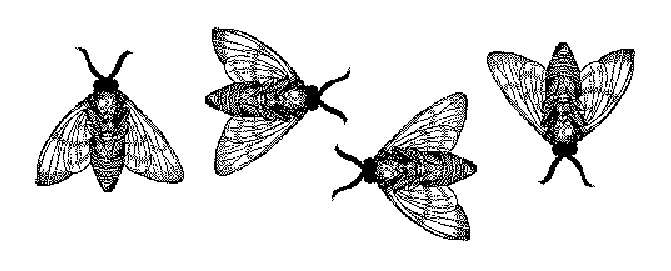
\epsfig{file=flies.eps}
\caption{A sample black and white graphic (.eps format)
that needs to span two columns of text.}
\end{figure*}
and don't forget to end the environment with
{figure*}, not {figure}!
 
There is one other similar construct environment, which is
already set up
for you; i.e. you must \textit{not} use
a \texttt{{\char'134}newdef} command to
create it: the \textbf{proof} environment.  Here
is a example of its use:
\begin{proof}
Suppose on the contrary there exists a real number $L$ such that
\begin{displaymath}
\lim_{x\rightarrow\infty} \frac{f(x)}{g(x)} = L.
\end{displaymath}
Then
\begin{displaymath}
l=\lim_{x\rightarrow c} f(x)
= \lim_{x\rightarrow c}
\left[ g{x} \cdot \frac{f(x)}{g(x)} \right ]
= \lim_{x\rightarrow c} g(x) \cdot \lim_{x\rightarrow c}
\frac{f(x)}{g(x)} = 0\cdot L = 0,
\end{displaymath}
which contradicts our assumption that $l\neq 0$.
\end{proof}

Complete rules about using these environments and using the
two different creation commands are in the
\textit{Author's Guide}; please consult it for more
detailed instructions.  If you need to use another construct,
not listed therein, which you want to have the same
formatting as the Theorem
or the Definition\cite{salas:calculus} shown above,
use the \texttt{{\char'134}newtheorem} or the
\texttt{{\char'134}newdef} command,
respectively, to create it.

\subsection*{A {\secit Caveat} for the \TeX\ Expert}
Because you have just been given permission to
use the \texttt{{\char'134}newdef} command to create a
new form, you might think you can
use \TeX's \texttt{{\char'134}def} to create a
new command: \textit{Please refrain from doing this!}
Remember that your \LaTeX\ source code is primarily intended
to create camera-ready copy, but may be converted
to other forms -- e.g. HTML. If you inadvertently omit
some or all of the \texttt{{\char'134}def}s recompilation will
be, to say the least, problematic.

\section{Conclusions}
This paragraph will end the body of this sample document.
Remember that you might still have Acknowledgments or
Appendices; brief samples of these
follow.  There is still the Bibliography to deal with; and
we will make a disclaimer about that here: with the exception
of the reference to the \LaTeX\ book, the citations in
this paper are to articles which have nothing to
do with the present subject and are used as
examples only.
%\end{document}  % This is where a 'short' article might terminate

%ACKNOWLEDGMENTS are optional
\section{Acknowledgments}
This section is optional; it is a location for you
to acknowledge grants, funding, editing assistance and
what have you.  In the present case, for example, the
authors would like to thank Gerald Murray of ACM for
his help in codifying this \textit{Author's Guide}
and the \textbf{.cls} and \textbf{.tex} files that it describes.

%
% The following two commands are all you need in the
% initial runs of your .tex file to
% produce the bibliography for the citations in your paper.
\bibliographystyle{abbrv}
\bibliography{sigproc}  % sigproc.bib is the name of the Bibliography in this case
% You must have a proper ".bib" file
%  and remember to run:
% latex bibtex latex latex
% to resolve all references
%
% ACM needs 'a single self-contained file'!
%
%APPENDICES are optional
%\balancecolumns
\appendix
%Appendix A
\section{Headings in Appendices}
The rules about hierarchical headings discussed above for
the body of the article are different in the appendices.
In the \textbf{appendix} environment, the command
\textbf{section} is used to
indicate the start of each Appendix, with alphabetic order
designation (i.e. the first is A, the second B, etc.) and
a title (if you include one).  So, if you need
hierarchical structure
\textit{within} an Appendix, start with \textbf{subsection} as the
highest level. Here is an outline of the body of this
document in Appendix-appropriate form:
\subsection{Introduction}
\subsection{The Body of the Paper}
\subsubsection{Type Changes and  Special Characters}
\subsubsection{Math Equations}
\paragraph{Inline (In-text) Equations}
\paragraph{Display Equations}
\subsubsection{Citations}
\subsubsection{Tables}
\subsubsection{Figures}
\subsubsection{Theorem-like Constructs}
\subsubsection*{A Caveat for the \TeX\ Expert}
\subsection{Conclusions}
\subsection{Acknowledgments}
\subsection{Additional Authors}
This section is inserted by \LaTeX; you do not insert it.
You just add the names and information in the
\texttt{{\char'134}additionalauthors} command at the start
of the document.

\subsection{References}
Generated by bibtex from your ~.bib file.  Run latex,
then bibtex, then latex twice (to resolve references)
to create the ~.bbl file.  Insert that ~.bbl file into
the .tex source file and comment out
the command \texttt{{\char'134}thebibliography}.

% This next section command marks the start of
% Appendix B, and does not continue the present hierarchy
\section{More Help for the Hardy}
The acm\_proc\_article-sp document class file itself is chock-full of succinct
and helpful comments.  If you consider yourself a moderately
experienced to expert user of \LaTeX, you may find reading
it useful but please remember not to change it.
\balancecolumns
% That's all folks!
\end{document}
